\subsection{Level3.1: パラメータのチューニング}%
\subsubsection{最適なパラメータを探すためのアプローチ}
指定された条件下において学習が効率良く行われるパラメータの組み合わせを探
すため、
hiddenを10から100まで10づつ増やしていき,etaを0.01から1.98まで0.01づつ増
やし,alphaを0.1から1.0まで0.1づつ増やしていきその中から一番値が小さい物
を探した.その動作をスクリプトを書いて実行させた.
その後その値の近辺をスクリプトで探した.
\subsubsection{実行結果}
各パラメータがeta = 1.95, ALPHA = 0.62, HIDDEN 30の時,表5のよ
うな結果が得られたその時の学習曲線の平均はerrorを一回の学習ごとに足し,
それをまだ終了していないパターンの個数で割って出した.例えば61回目の学習
でシード値10000のパターンは収束しているので62回目の場合はerrorを足して9で
割ることで平均をだした.
\begin{table}[htb]
 \begin{center}
  \caption{階層型NNによる文字認識問題の学習に要した回数}
  \label{table:level3}
  \begin{tabular}[htb]{r|l} \hline
   シード値 & 収束した回数 \\ \hline \hline
   1000 & 105 \\ \hline
   2000 & 75 \\ \hline
   3000 & 62 \\ \hline
   4000 & 126 \\ \hline
   5000 & 74 \\ \hline
   6000 & 87 \\ \hline
   7000 & 85 \\ \hline
   8000 & 78 \\ \hline
   9000 & 122 \\ \hline
   10000 & 61 \\ \hline \hline
   10試行の平均値 & 87.5 \\ \hline
  \end{tabular}
 \end{center}
\end{table}

\begin{figure}[h]
 \begin{center}
  \includegraphics[width=10.0cm]{./figs/average.eps}
  \caption{重みを更新する様子(平均値)}
  \label{fig:level2}
 \end{center}
\end{figure}
\newpage


